\chapter{الدماغ في القيادة}\label{ch:g5:brain-in-command}

كرة تطير نحوك؛ فتلقفها. نصف ثانية، بلا تفكير البتة --- ومع ذلك
ففي ذلك النصف من الثانية بلّغت عيناك عن جسم طائر، وحسب شيء ما
مساره، وأُمرت عشرات \omterm{def:g3:bones-and-muscles:muscle}{العضلات} باللقفة الصحيحة تمامًا. وذلك الشيء هو
\omterm{def:g5:brain-in-command:system}{الدماغ}، وهذا الفصل يتتبع أوامره على أسلاك الجسم.

\section{شبكة القيادة}

\begin{definition}[الجهاز العصبي]\label{def:g5:brain-in-command:system}
\emph{الجهاز العصبي}\index{جهاز عصبي} شبكة القيادة في الجسم:
\begin{itemize}
  \item \emph{الدماغ}\index{دماغ}، في حمى \omterm{def:g3:bones-and-muscles:skeleton}{الجمجمة}
        (\cref{def:g3:bones-and-muscles:skeleton})، هو المركز:
        يتلقى كل التقارير ويصدر كل الأوامر؛
  \item و\emph{النخاع الشوكي}\index{نخاع شوكي}، وهو كبل غليظ من
        نسيج عصبي، ينزل من الدماغ داخل عمود \omterm{def:g3:bones-and-muscles:skeleton}{العمود الفقري}
        الواقي؛
  \item و\emph{الأعصاب}\index{عصب}، وهي خيوط بيضاء تتفرع من
        الدماغ والنخاع الشوكي إلى كل عضو، تحمل الرسائل ---
        بأكثر من \qty{100}{m/s} في أسرعها.
\end{itemize}
\end{definition}

\begin{proposition}[تبليغ وقرار وأمر]\label{prop:g5:brain-in-command:loop}
كل فعل يجري في الحلقة نفسها
(وكانت \cref{prop:g1:the-five-senses:brain} رسمها الأول):
\begin{enumerate}
  \item \emph{\omterm{def:g1:the-five-senses:sense}{أعضاء الحس}} تبلّغ: \omterm{def:g5:brain-in-command:system}{فالأعصاب} تحمل رسائلها
        \emph{إلى} \omterm{def:g5:brain-in-command:system}{الدماغ}؛
  \item و\emph{\omterm{def:g5:brain-in-command:system}{الدماغ}} يجمع التقارير، ويقرر، ويؤلّف الأوامر؛
  \item \omterm{def:g5:brain-in-command:system}{والأعصاب} تحمل الأوامر \emph{من} \omterm{def:g5:brain-in-command:system}{الدماغ} إلى
        \emph{\omterm{def:g3:bones-and-muscles:muscle}{العضلات}} (\cref{def:g3:bones-and-muscles:muscle})،
        وهي \omterm{def:g3:bones-and-muscles:muscle}{تنقبض} بالأمر.
\end{enumerate}
\omterm{def:g1:the-five-senses:sense}{فأعضاء الحس} تبلّغ، \omterm{def:g3:bones-and-muscles:muscle}{والعضلات} تطيع --- ولا واحدة منهما تقرر أبدًا.
\end{proposition}
\admitted

\begin{omfigure}
\begin{tikzpicture}
  % eye
  \draw[thick] (-0.7,1.7) ellipse (0.5 and 0.28);
  \fill[omDef] (-0.58,1.7) circle (0.13);
  \node[font=\small, align=center] (eye) at (-0.7,0.85)
    {العين ترى\\ الكرة};
  % brain
  \draw[thick, omDef, fill=omDef!8, rounded corners=8pt]
    (3.2,1.15) rectangle (6.4,2.45);
  \node[font=\small\bfseries, omDef] at (4.8,2.05) {الدماغ};
  \node[font=\footnotesize] at (4.8,1.55) {يقرر اللقف};
  % muscle
  \draw[thick, omThm, fill=omThm!15]
    (9.6,1.5) .. controls (10.0,1.85) and (10.6,1.85) .. (11.0,1.55)
    .. controls (10.6,1.35) and (10.0,1.35) .. (9.6,1.5);
  \node[font=\small, align=center] at (10.3,0.85)
    {عضلات الذراع\\ تنقبض};
  % arrows
  \draw[->, very thick, omMeth] (-0.1,1.7) -- (3.1,1.8)
    node[pos=0.42, above=2pt, font=\footnotesize, omMeth]
    {تبليغ في عصب};
  \draw[->, very thick, omProp] (6.5,1.8) -- (9.5,1.6)
    node[pos=0.5, above=2pt, font=\footnotesize, omProp]
    {أمر في عصب};
\end{tikzpicture}

{\small حلقة كل فعل: تبليغ إلى \omterm{def:g5:brain-in-command:system}{الدماغ}، فقرار، فأمر إلى \omterm{def:g3:bones-and-muscles:muscle}{العضلات}.}
\end{omfigure}

\begin{example}[اللقفة معادةً ببطء]\label{ex:g5:brain-in-command:catch}
أعد نصف الثانية: \omterm{def:g1:the-five-senses:sense}{العينان} تتتبعان الكرة وتبلّغان باستمرار؛ \omterm{def:g5:brain-in-command:system}{والدماغ}،
إذ يقارن تقريرًا بتقرير، يستنتج أين ستكون الكرة؛ وتنهمر الأوامر إلى
\omterm{def:g1:my-body:parts}{الرجلين} (خطوة إلى اليسار)، \omterm{def:g1:my-body:parts}{والبدن} (ميلًا)، \omterm{def:g1:my-body:parts}{والذراع} والأصابع (افتح
--- والآن أغلق). فلم ``يلقف الكرة'' عضو واحد: بل أدّت \omterm{def:g1:the-five-senses:sense}{العينان}
\omterm{def:g5:brain-in-command:system}{والدماغ} \omterm{def:g3:bones-and-muscles:muscle}{والعضلات} كل منها دوره في
\cref{prop:g5:brain-in-command:loop}.
\end{example}

\begin{remark}[أكثر من الحركة]\label{rem:g5:brain-in-command:more}
\omterm{def:g5:brain-in-command:system}{والدماغ} نفسه الذي يلقف الكرات يخزن ذكرياتك أيضًا، ويثبّت انتباهك
على هذه الصفحة، ويحلم في الليل --- ويدير خدمات لا تفكر فيها قط:
فهو يُبقي \omterm{def:g4:breathing:movements}{التنفس} ماضيًا ليلًا ونهارًا
(\cref{def:g4:breathing:movements})، ويضبط وتيرة \omterm{def:g4:heart-and-blood:heart}{القلب} على حاجات
الجسم (\cref{ex:g4:heart-and-blood:effort}). فبعض الأوامر لك أن
تصدرها؛ وبعضها يصدره \omterm{def:g5:brain-in-command:system}{الدماغ} عنك.
\end{remark}

\section{قياس الحلقة: زمن رد الفعل}

\begin{definition}[زمن رد الفعل]\label{def:g5:brain-in-command:reaction}
الحلقة سريعة لكنها ليست فورية: فالتبليغ والقرار والأمر يأخذ كل
واحد منها حصته. والتأخير بين إشارة واستجابة الجسم لها هو
\emph{زمن رد الفعل}\index{زمن رد الفعل} --- وهو في مهمة بسيطة
(لقف، أو ضغط، أو إمساك) نحو خُمس ثانية عند المتمرن، وأكثر قليلًا
عند الأطفال.
\end{definition}

\begin{method}[اختبار المسطرة]\label{met:g5:brain-in-command:ruler}
\omterm{def:g5:brain-in-command:reaction}{زمن رد الفعل} بلا آلة سوى مسطرة:
\begin{enumerate}
  \item يمسك شريك مسطرة متدلية عموديًّا، وعلامة الصفر إلى أسفل،
        بين إبهامك وإصبعك المفتوحين؛
  \item ثم يفلتها من غير إنذار؛ فتلقفها بأسرع ما تستطيع؛
  \item واقرأ عند أي موضع لقفتها: فكلما قلّت السنتيمترات التي
        انزلقت، كانت حلقتك أسرع؛
  \item وأعد ذلك مرات عدة واحتفظ بقيمتك المعتادة --- فالمحاولات
        المفردة تقفز هنا وهناك.
\end{enumerate}
والمسطرة الساقطة تحوّل الزمن سنتيمترات: فنحو $\qty{15}{cm}$ يقابل
سدس ثانية.
\end{method}

\begin{omfigure}
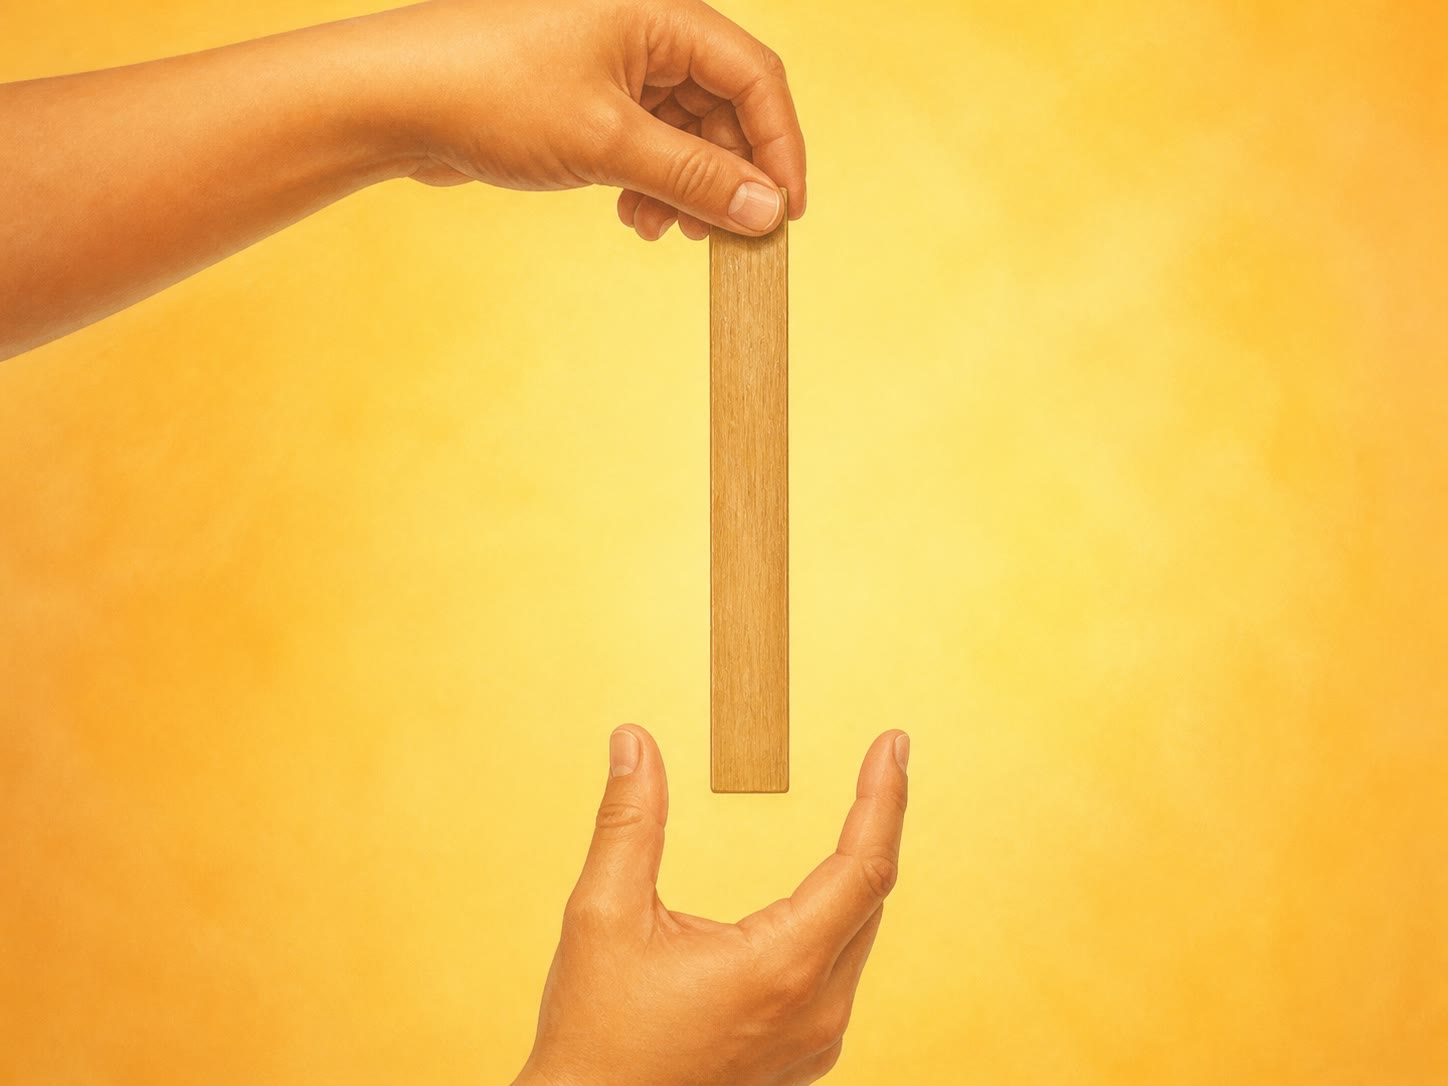
\includegraphics[width=0.5\linewidth]{images/book1/ai/g5-brain-ruler.jpg}

{\small اختبار المسطرة قبل الإفلات بلحظة: فحين تفلتها اليد العليا،
تبدأ حلقة اليد السفلى --- ترى، وتقرر، وتغلق --- خُمس ثانيتها.}
\end{omfigure}

\begin{example}[لماذا يلهث مقعد الراكب أولًا]\label{ex:g5:brain-in-command:driver}
خُمس الثانية يبدو لا شيء --- إلى أن تضاعفه السرعة. فالسيارة على
سرعة الطريق السريع تقطع نحو \qty{7}{m} في خُمس ثانية من رد الفعل:
فالسائق لم يمسّ المكبح بعد، والسيارة قد عبرت صفًّا دراسيًّا. \omterm{def:g5:brain-in-command:reaction}{وزمن رد
الفعل} هو سبب وجود المسافات بين السيارات، وسبب كون انتباه السائق
عضوًا من أعضاء السلامة.
\end{example}

\begin{remark}[تمرين الحلقة]\label{rem:g5:brain-in-command:training}
التمرين يقصّر الحلقة ويشحذها --- لا سرعة \omterm{def:g5:brain-in-command:system}{الأعصاب}، بل توجيه \omterm{def:g5:brain-in-command:system}{الدماغ}.
فالمشعوذ المبتدئ يُسقط كل شيء؛ وبعد شهر يأمر \omterm{def:g5:brain-in-command:system}{الدماغ} نفسه اليدين
نفسيهما بثلاث كرات بلا جهد ظاهر. وتعلّم مهارة هو أن يمدّ \omterm{def:g5:brain-in-command:system}{الدماغ}
مسالك أفضل --- وهو شيء آخر ينمو بالتمرين، \omterm{def:g3:bones-and-muscles:muscle}{كعضلات}
\cref{met:g3:bones-and-muscles:care}.
\end{remark}

\section{حماية القائد}

\begin{proposition}[النوم والغذاء والسلامة]\label{prop:g5:brain-in-command:protect}
\omterm{def:g5:brain-in-command:system}{الدماغ} أشدّ أعضاء الجسم حمايةً --- خوذة \omterm{def:g3:bones-and-muscles:skeleton}{الجمجمة}، وعمود \omterm{def:g3:bones-and-muscles:skeleton}{العمود
الفقري} --- وأكثرها طلبًا: فهو، وإن كان جزءًا صغيرًا من وزن الجسم،
يستهلك حصة كبيرة من طاقته وأكسجينه
(\cref{prop:g4:heart-and-blood:carries})، ويقوم بحفظ ملفاته
وإصلاحاته في أثناء \emph{\omterm{prop:g1:healthy-habits:needs}{النوم}}
(\cref{prop:g1:healthy-habits:needs}). \omterm{def:g5:brain-in-command:system}{والدماغ} المتعب يقود قيادة
سيئة: ردود أفعال أبطأ، وانتباه مشتَّت، وقرارات متبرّمة.
\end{proposition}
\admitted

\begin{example}[الخوذ من أجل الحلقة]\label{ex:g5:brain-in-command:helmet}
\omterm{def:g3:bones-and-muscles:skeleton}{العظام} تلتئم (\cref{rem:g3:bones-and-muscles:alive})؛ أما نسيج
\omterm{def:g5:brain-in-command:system}{الدماغ} فلا يلتئم في أكثره متى أُصيب إصابة بالغة. وذلك هو الحساب
وراء خوذ الدراجات: \omterm{def:g3:bones-and-muscles:skeleton}{جمجمة} مع إسفنج حيث قد لا تكفي حماية الجسم
نفسها. تأمين رخيص للعضو الذي يدير كل ما عداه.
\end{example}

\section{تمارين}

\begin{exercise}[$\star$]\label{exo:g5:brain-in-command:1}
سمِّ أجزاء \omterm{def:g5:brain-in-command:system}{الجهاز العصبي} الثلاثة ودور كل واحد.
\end{exercise}

\begin{exercise}[$\star$]\label{exo:g5:brain-in-command:2}
اذكر حلقة كل فعل في ثلاث خطوات. وأي الأجزاء تبلّغ، وأيها يقرر،
وأيها يطيع؟
\end{exercise}

\begin{exercise}[$\star$]\label{exo:g5:brain-in-command:3}
أين يُحمى \omterm{def:g5:brain-in-command:system}{الدماغ} وأين يُحمى \omterm{def:g5:brain-in-command:system}{النخاع الشوكي}، وبأي \omterm{def:g3:bones-and-muscles:skeleton}{عظام}؟
\end{exercise}

\begin{exercise}[$\star$]\label{exo:g5:brain-in-command:4}
ما \omterm{def:g5:brain-in-command:reaction}{زمن رد الفعل}؟ أعطِ قيمته التقريبية في مهمة بسيطة.
\end{exercise}

\begin{exercise}[$\star$]\label{exo:g5:brain-in-command:5}
أعد الحكاية ببطء، كما في \cref{ex:g5:brain-in-command:catch}: تدوس
على شيء حادّ فتنتفض قدمك بعيدًا. فمن بلّغ، ومن قرر، ومن أطاع؟
\end{exercise}

\begin{exercise}[$\star$]\label{exo:g5:brain-in-command:6}
اذكر خدمتين يديرهما \omterm{def:g5:brain-in-command:system}{الدماغ} من غير أن تفكر فيهما، من
\cref{rem:g5:brain-in-command:more}.
\end{exercise}

\begin{exercise}[$\star$]\label{exo:g5:brain-in-command:7}
لماذا يقود \omterm{def:g5:brain-in-command:system}{الدماغ} المتعب قيادة سيئة؟ سمِّ حاجتين من حاجاته في
\cref{prop:g5:brain-in-command:protect}.
\end{exercise}

\begin{exercise}[$\star$]\label{exo:g5:brain-in-command:8}
جرّب: أجرِ اختبار المسطرة في
\cref{met:g5:brain-in-command:ruler}، خمس محاولات. واذكر مسافة
لقفك المعتادة --- وهل حسّنها التمرين.
\end{exercise}

\begin{exercise}[$\star\star$]\label{exo:g5:brain-in-command:9}
لماذا لا توجد لقفة فورية مهما تكن مهارة اللاقف؟ أجب بخطوات الحلقة
الثلاث.
\end{exercise}

\begin{exercise}[$\star\star$]\label{exo:g5:brain-in-command:10}
مستعملًا \cref{ex:g5:brain-in-command:driver}: لماذا تطلب قواعد
المرور \emph{مسافة} بين السيارات لا مجرد مكابح جيدة؟ وما الذي
يغيّره الانتباه في الحلقة؟
\end{exercise}

\begin{exercise}[$\star\star\star$]\label{exo:g5:brain-in-command:11}
تحسّنت المشعوذة في \cref{rem:g5:brain-in-command:training} من غير
أن تصير أعصابها أسرع نقلًا. فأي جزء من الحلقة تحسّن بدل ذلك؟ قارن
بتمرين \omterm{def:g3:bones-and-muscles:muscle}{عضلة}: ما الذي ينمو في كل حالة؟
\end{exercise}
